 % !TEX encoding = UTF-8 Unicode
\documentclass[a4paper,11pt]{article}

%% LaTeX Preamble - Common packages
\usepackage[a4paper]{geometry}
%\usepackage[left=2cm,right=2cm,top=2cm,bottom=2cm]{geometry}

\usepackage[utf8]{inputenc} % Any characters can be typed directly from the keyboard, eg éçñ
\usepackage[T1]{fontenc}

\usepackage{textcomp} % provide lots of new symbols
\usepackage{graphicx}  % Add graphics capabilities
%\usepackage{epstopdf} % to include .eps graphics files with pdfLaTeX
\usepackage{flafter}  % Don't place floats before their definition
%\usepackage{topcapt}   % Define \topcation for placing captions above tables (not in gwTeX)

\usepackage{amsmath,amssymb,amsthm}  % Better maths support & more symbols
\usepackage[french]{babel}

\usepackage{algorithm}
\usepackage{algorithmic}


%Nouvelles commandes
\newcommand{\real}{\mathbb{R}}
\newcommand{\ha}{\hat{A}}
\newcommand{\hc}{\hat{c}}

% écart interline
\usepackage{setspace}
\onehalfspacing

\numberwithin{equation}{section}

\usepackage[pdftex,bookmarks,colorlinks,breaklinks]{hyperref}  % PDF hyperlinks, with coloured links


\hypersetup{linkcolor=black,citecolor=blue,filecolor=dullmagenta,urlcolor=darkblue} % coloured links
%\hypersetup{linkcolor=black,citecolor=black,filecolor=black,urlcolor=black} % black links, for printed output

\usepackage{memhfixc}  % remove conflict between the memoir class & hyperref
% \usepackage[activate]{pdfcprot}  % Turn on margin kerning (not in gwTeX)
\usepackage{pdfsync}  % enable tex source and pdf output syncronicity






\usepackage{pgfplots}
\usepackage{tikz}
\usepackage{color}

\newif\ifnotes\notestrue
%  \notesfalse     %%  Uncomment this line to hide footnotes.  <----
\def\perhaps#1{{\color{gray}#1\color{black}}}
\def\remove#1{{\color{gray}\sout{#1}\color{black}}}
%
\def\boxnote#1#2{\ifnotes\fbox{\footnote{\ }}\ \footnotetext{ From #1: #2}\fi}
%
\def\pierre#1{\boxnote{Pierre}{\color{red}#1}}
\def\mpierre#1{{\color{red} #1}}
% \def\mpierre#1{#1}
\def\hpierre#1{}

\def\fabian#1{\boxnote{Fabian}{\color{blue}#1}}
\def\mfabian#1{{\color{blue} #1}}
% \def\mpierre#1{#1}
\def\hfabian#1{}




\begin{document}

\title{Rapport de stage d'Insertion Professionnelle: \\ Transcription de l'algorithme ENLSIP en Julia}
\author{Pierre Borie \\ ENAC}

\date{8 Juin 2020 -11 Septembre 2020}
\maketitle



	
\begin{abstract}
J'ai effectué mon stage d'insertion professionnelle pour HydroQuebec transénergie, plus précisément la division de prévision de la demande, en collaboration avec Mr Fabian Bastin de l'Université de Montréal, qui était mon maître de stage. J'ai travaillé sur la transcription de l'algorithme d'optimisation ENLSIP. Cet algorithme, initialement codé en Fortran77, est utilisé en production afin de prédire la demande en électricité dans une période de 24 heures. Ce rapport illustre les résultats de mes travaux sur la compréhension du fonctionnement de l'algorithme et sur son implémentation en Julia. J'ai été en télétravail depuis la France durant la totalité de mon stage. 
\end{abstract}

\tableofcontents

\section{Introduction} \label{intro}
\subsection{Présentation du problème à résoudre} \label{presentation}


Pour la suite, $q,l,m\text{ et }n$ sont des entiers naturels tels que $q \leq l \leq n \leq m$. 

On dispose de $m$ observations réelles $(t_{i},y_{i})$ et l'on souhaite ajuster un modèle $h$ paramétré par $x\in \mathbb{R}^{n}$ qui approche au mieux nos observations, le tout en satisfaisant $l$ contraintes, dont $q$ sont des contraintes d'égalité. Pour cela, on cherche le paramètre $x^{*}$ qui minimise la somme des écarts entre prédictions et observations au carré, soit:\fabian{Ne pas mettre d'espace avant le ':' en \LaTeX, qui s'en chargera.}
\[
\underset{x \in \mathbb{R}^{n}}{\min} \sum_{i=1}^{m} \left(h(t_{i},x)-y_{i})\right)^{2}
\]
Pour $i=1,\ldots,m$, $r_{i}: x \to y_{i} - h(t_{i},x)$ est le $i$-ème résidu.
L'algorithme sur lequel j'ai travaillé a pour finalité la résolution d'un problème d'optimisation de la forme:\fabian{Dans l'équation, il est préférable d'éviter l'environnement array, et privilégier align et la commande matrix.}
\begin{equation} \label{pb}
\left\{ \begin{array}{l l l l} \underset{x \in \mathbb{R}^n}{\min}  \dfrac{1}{2}\|r(x)\|^2 \\ 
\textnormal{sous contraintes} \\
c_{i}(x) = 0& i=1,\ldots,q 
\\ c_{j}(x) \geq 0& j=q+1,\ldots,l  \end{array} \right. 
\end{equation}

On a $r =(r_{1}, \ldots,r_{m}): \mathbb{R}^{n} \mapsto \mathbb{R}^{m}$ la multi-fonction vectorielle des résidus et $c = (c_{1}, \ldots, c_{l})^{T}: \mathbb{R}^{n} \mapsto \mathbb{R}^{l}$\fabian{Pourquoi la transposition pour $c$ mais pas pour $r$?} multi-fonction des contraintes dont les $q$ premières composantes sont des contraintes d'égalité et les $l-q$ suivantes sont des contraintes d'inégalité. On suppose les $r_{i}$ et $c_{j}$ deux fois continûment différentiables.  

$f:x\mapsto \dfrac{1}{2}\|r(x)\|^{2}$ est la fonction objectif à minimiser.

\subsection{Idée générale de la résolution}

L'algorithme implémenté est un algorithme itératif où, partant d'un point $x_{0}$,  à une itération $k$, on calcule:
\begin{itemize}
\item
$p_{k} \in \real^{n}$ une direction de descente
\item
$\alpha_{k} \in \real$ une longueur de pas
\end{itemize}
Et\fabian{Ne pas commencer une phrase par 'Et'.} on met à jour le point courant par la relation: 

\begin{equation}
x_{k+1} = x_{k}+\alpha_{k}p_{k}
\end{equation}
 
\section{Calcul de la direction de descente}



\subsection{Méthode de Gauss-Newton} \label{method:gn}
\subsubsection{Modélisation du sous-problème} \label{gn:model}

Les explications ci-dessous se basent sur celles fournies dans \cite{lindstromwedin1988}.

Soit $\tilde{x}$ une approximation de la solution du problème \ref{pb}. Dans un voisinage $\delta x$, à partir du développement de Taylor d'ordre 1, on a, pour $i=1,\ldots,m$, l'approximation suivante du $i$-ème résidu:

\begin{equation}
r_{i}(\tilde{x} + \delta x) \approx r_{i}(\tilde{x}) + \left(\dfrac{\partial r_{i}(\tilde{x})}{\partial x_{1}}, \ldots, \dfrac{\partial r_{i}(\tilde{x})}{\partial x_{n}}\right)\delta x 
\end{equation}

De même pour la $j$-ième contrainte, $j=1,\ldots,l$: 

\begin{equation}
c_{j}(\tilde{x} + \delta x) \approx c_{j}(\tilde{x}) + \left(\dfrac{\partial c_{j}(\tilde{x})}{\partial x_{1}}, \ldots, \dfrac{\partial c_{j}(\tilde{x})}{\partial x_{n}}\right)\delta x 
\end{equation}

Ce qui, en notant $J$ et $A$ les matrices jacobiennes respectives des multi-fonctions $r$ et $c$, donne les linéarisations:
\begin{eqnarray} 
r(\tilde{x}+\delta x) &=& J(\tilde{x})\delta x + r(\tilde{x}) \label{linearisationr}\\
c(\tilde{x}+\delta x) &=& A(\tilde{x})\delta x + c(\tilde{x}) \label{linearisationc}
\end{eqnarray}

Ces linéarisations seront injectées dans la formulation du problème \ref{pb} mais avant, nous allons nous intéresser à la considération des contraintes.

L'idée est, à une itération donnée, d'estimer quelles sont les contraintes actives\fabian{Les contraintes d'égalité sont, par définition, actives. Ce sont les contraintes d'inégalité qui posent problème.} qui peuvent donc être traitées comme des égalités. L'ensemble de ces contraintes, aussi appelé ensemble de travail et noté $\mathcal{W}$, peut être vu comme une prédiction de l'ensemble actif final, i.e. toutes les contraintes nulles à la solution\fabian{Cela ne tient que si on a des qualifications de contraintes adéquates, probablement la LICQ, et aussi la complémentarité stricte. Quelles sont les hypothèses de l'article?}. Parmi ces contraintes on retrouve évidemment les contraintes d'égalité\fabian{Cela devrait être dit avant.}, qui sont par définition actives, et certaines contraintes d'inégalité. Les autres contraintes ne sont pas prises en compte dans le calcul\fabian{Quel calcul?}. 

\mfabian{La détermination de l'ensemble $\mathcal{W}$ sera détaillée dans la section~\ref{working-set}). L}e lagrangien du problème\mfabian{ s'écrit comme} 
\begin{equation} \label{lagrangien}
\mathcal{L}:(x,\lambda) \mapsto f(x) - \sum\limits_{i\in \mathcal{W}} \lambda_{i}c_{i}(x)
\end{equation}

Les composantes du vecteur $\lambda$ désignent les multiplicateurs de Lagrange. C'est à partir de leurs valeurs, en particulier du signe des multiplicateurs associés aux inégalités, que l'ensemble $\mathcal{W}$ est mis à jour au début de chaque nouvelle itération.

Finalement, tout cela implique que l'on réduit le nombre de contraintes considérées à $t$ $(q \leq t \leq l)$. 

Parmi ces $t$ contraintes, on retrouve:
\begin{itemize}
\item
toutes les contraintes d'égalité
\item
les contraintes d'inégalité actives considérées comme des contraintes d'égalité. \fabian{Je crois comprendre un peu mieux la distinction entre ensemble de travail et ensemble actif. L'ensemble actif reprend les contraintes actives au point courant, tandis que l'ensemble de travail ne contient que les contraintes qui vont rester actives.}
\end{itemize}

On note $\hc$ la restriction de $c$ à $t$ composantes et $\ha$ sa matrice jacobienne. La linéarisation \ref{linearisationc} de $c$ reste valable pour $\hc$.

A l'itération $k$,  le point courant $x_{k}$, les vecteurs $r(x_{k})$ et $\hc(x_{k})$ ainsi que les matrices $J_{k}=J(x_{k}) \text{ et } \ha_{k}=\ha(x_{k})$ sont fixés. On cherche alors la direction de descente $p_{k}$ qui nous rapproche au mieux du minimum de la fonction objectif. En injectant les linéarisations de $r$ et $\hc$, on obtient le sous-problème suivant:

\begin{equation} \label{souspb}
\left\{ \begin{array}{l l l}
\underset{p \in \real^{n}}{\min} \dfrac{1}{2}\|J_{k}p+r(x_{k})\|^{2} \\
\text{s.c.} \\
\ha_{k}p+\hc(x_{k})=0
\end{array} \right.
\end{equation}
C'est-à-dire un problème de moindres carrés linéaires sous contraintes d'égalité linéaires.

\subsubsection{Factorisation QR} \label{factqr}

Le c\oe ur de la résolution du problème \ref{souspb} réside dans la factorisation QR de différentes matrices.  On rappelle ci-dessous la factorisation QR d'une matrice disposant de plus de lignes que de colonnes.

\newtheorem*{theo}{Théorème}
\begin{theo}[Factorisation QR]
Soit $M \in \mathcal{M}_{m\times n}$ avec $m$ et $n$ des entiers quelconques tel que $m\geq n$.

Alors il existe $Q\text{ une matrice orthogonale } m\times m$, $ R \text{ de taille }n \times n$ une matrice triangulaire supérieure et $P \text{ une matrice de permutation } n\times n$ tel que:
\[
MP = Q 
\begin{pmatrix} 
R \\ 
0
\end{pmatrix}
\]
avec $|r_{11}| \geq |r_{22}| \geq \ldots \geq |r_{nn}|$ où les $r_{ii}$ désignent les éléments diagonaux de $R$. 
\end{theo}

Cette factorisation n'est pas unique mais dispose de nombreux avantages pratiques pour les problèmes de moindres carrés, ce que nous verrons tout au long de ce \mfabian{document}. Notons d'ores et déjà que la décomposition ci-dessus est très facile à obtenir en Julia puisqu'il suffit d'appliquer la fonction \texttt{qr} du package \texttt{LinearAlgebra} à la matrice que l'on souhaite factoriser. \mfabian{U}n argument optionnel permet même d'obtenir directement la matrice de permutation associée.

\subsubsection{Décomposition en sous-systèmes}

On souhaite d'abord factoriser la matrice $\ha_{k}$ de taille $t \times n$ mais comme $t \leq n$, on passe par la factorisation QR de $\ha_{k}^{T}$:
\begin{equation} \label{qrAt}
\ha_{k}^{T}P_{1}=Q_{1}
\begin{pmatrix}
R_{1} \\
0
\end{pmatrix}
\end{equation}
avec: \begin{itemize}
\item
$Q_{1}\text{ matrice orthogonale } n\times n$, 
\item
$ R_{1} \text{ matrice triangulaire supérieure } t \times t$ à éléments diagonaux décroissants en valeur absolue
\item
$P_{1} \text{ matrice de permutation } n\times n$
\end{itemize}

\textbf{\underline{N.B.}}: Les matrices issues de la décomposition QR ci-dessus ne sont pas indexées par $k$ par soucis de lisibilité mais sont bien dépendantes de l'itération en cours. Il en va de même pour les différentes factorisations QR présentées dans la suite de ce papier.

Par transposition et par le fait que $P_{1}P_{1}^{T} = I_{t}$, on obtient:
\begin{equation}
\ha_{k} = P_{1}
\begin{pmatrix}
L_{1} & 0
\end{pmatrix}
Q_{1}^{T}
\end{equation}

où $L_{1}=R_{1}^{T}$ est une matrice triangulaire inférieure $t \times t$.

Injectons cette factorisation l'équation des contraintes du problème \ref{souspb}: 
\[
\ha_{k}p = -c(x_{k}) \Longleftrightarrow P_{1}\begin{pmatrix}
L_{1} & 0
\end{pmatrix}
Q_{1}^{T}p = -c(x_{k})
\]

Posant $Q_{1}^{T}p = \begin{pmatrix}
p_{1} \\ p_{2}
\end{pmatrix}$ avec $p_{1} \in \real^{t}$ et $p_{2} \in \real^{n-t}$ , on a:
\[
P_{1}L_{1}p_{1} = -\hc(x_{k}) \Longleftrightarrow L_{1}p_{1} = -P_{1}^{T}\hc(x_{k}) = b
\]

On remarque que $p_{1}$, soit les $t$ premiers éléments de $p$, est totalement déterminé par les contraintes tandis que $p_{2}$, soit les $n-t$ derniers éléments de $p$, peut être choisi librement. Cela se comprend en introduisant l'espace nul de $\ha_{k}$. Notons $Y$ le bloc des $t$ premières colonnes de $Q_{1}$ et $Z$ celui des $n-t$ dernières;  on a $AZ=0$ d'où:

$$
Ap = AQ_{1} \begin{pmatrix}
p_{1}\\p_{2}
\end{pmatrix}=AYp_{1}
$$

La stratégie va maintenant être de calculer $p_{1}$ par rapport aux contraintes puis, $p_{1}$ fixé, de calculer $p_{2}$ de sorte à minimiser la fonction objectif du problème \mfabian{linéarisé \eqref{souspb}}. En injectant $p_{1}$ et $p_{2}$ dans cette dernière, on peut alors décomposer notre problème en deux nouveaux sous-problèmes:
\[
\left\{
\begin{array}{l l}
L_{1}p_{1} = b \\
\underset{p_{2}}{\min} \dfrac{1}{2}\|J_{2}p_{2} + J_{1}p_{1} + r(x_{k})\|^{2}
\end{array}\right.
\]
en introduisant $JQ_{1} = \begin{pmatrix}
J_{1} & J_{2}
\end{pmatrix}$, $J_{1} \in \mathcal{M}_{m\times t}$ et $J_{2} \in \mathcal{M}_{m\times (n-t)}$, puisque \\ $Jp=JQ_{1}Q_{1}^{T}p$.\mfabian{Ne sépare pas les équations du texte avec des espaces.}

Avant d'entamer les calculs, calculons le rang de $\ha_{k}$. Comme $Q_{1}$ et $P_{1}$ sont orthogonales, on a $\text{rang}(\ha_{k})=\text{rang}(L_{1})$ et $L_{1}$ étant triangulaire d'éléments diagonaux décroissants en valeur absolue, on définit son rang comme étant:
\begin{equation} \label{tbar}
\bar{t} = \underset{1\leq j\leq t}{\max} \left\{ j\ | \ |l_{jj}| \geq \varepsilon_{rank}\right\}
\end{equation} où $\varepsilon_{rank}$ est la racine carrée de la précision relative et les $l_{ii}$ sont les éléments diagonaux de $L_{1}$.

Cette valeur sera comparée au nombre de contraintes actives $t$ et modifiera la méthode de calcul de $p_{1}$\fabian{Expliqué dans une autre section?}.

\subsubsection{Résolution avec stabilisation}

Si $\bar{t}<t$, il faut réaliser ce qui est appelé dans \cite{lindstromwedin1988} une stabilisation\fabian{Pourquoi?}. Cela passe par la factorisation QR de $L_{1}$: 
\begin{equation} \label{qrL}
L_{1}P_2 = Q_{2} R_{2}
\end{equation}

avec:
\begin{itemize}
\item
$Q_2$ matrice orthogonale $t \times t$
\item
$R_{2}$ matrice triangulaire supérieure $t \times t$ à éléments diagonaux décroissants en valeur absolue 
\item
$P_2$ matrice de permutation $t \times t$
\end{itemize}

Le système d'inconnue $p_{1}$ devient alors:
$$ R_{2}P_2^Tp_1 = -Q_2^TP_1^Tc(x_{k}) = b_{1} $$ 
Pour $\omega_{1} \leq t$, on définit $R_{2}^{(\omega_{1})}$ comme le bloc triangulaire supérieur composé des $\omega_{1}$ premières lignes et colonnes de $R_{11}$ et $b_{1}^{(\omega_{1})}$ le vecteur des $\omega_{1}$ premiers éléments de $b_{1}$. Par suite, posant $\delta p_1^{(\omega_{1})}$ solution du système d'inconnue $y \in \real^{\omega_{1}}$  $R_{2}y=b_{1}^{(\omega_{1})}$, on obtient:
\begin{equation}
p_1 = P_2\begin{pmatrix} \delta p_1^{(\omega_{1})} \\ 0 \end{pmatrix}
\end{equation}
$p_1$ étant désormais calculé, il reste à résoudre pour $p_2$ $\underset{p_2}{\min} \dfrac{1}{2}\|J_2p_2 + (J_1P_{2}p_1 + r(x_{k}))\|^2$. 


On se sert alors de la factorisation QR de $J_{2}$:
\begin{equation} \label{qrJ2}
J_{2} = Q_3\begin{pmatrix} R_{3} \\ 0\end{pmatrix}P_3
\end{equation}

avec:
\begin{itemize}
\item
$Q_3$ matrice orthogonale $m \times m$
\item
$R_{3}$ matrice triangulaire supérieure $(n-t) \times (n-t)$ à éléments diagonaux décroissants en valeur absolue 
\item
$P_3$ matrice de permutation $(n-t) \times (n-t)$
\end{itemize}

On pose $d_{1} = -Q_3^T(r(x_{k}) + J_1P_{2}p_1)$ et pour $\omega_{2} \leq n-t$, on définit $R_{3}^{(\omega_{2} )}$ comme le bloc triangulaire supérieur composé des $\omega_{2}$ premières lignes et colonnes de $R_{3}$ et \\ $d_{1}^{(\omega_{2})} $ le vecteur constitué des $\omega_{2}$ premiers éléments de $d_{1}$.
Par suite, posant $\delta p_2^{(\omega_{2})}$ solution de $R_{3}^{(\omega_{2})}y =d^{(\omega_{2})}$, on obtient:
\begin{equation}
p_2 = P_3^T\begin{pmatrix} \delta p_2^{(\omega_{2})} \\ 0 \end{pmatrix}
\end{equation}
\subsubsection{Résolution sans stabilisation} \label{resolutionsstab}


Si $\bar{t}=t$, on résout directement le système $L_{1}p_{1}=b$ comme suit:

Pour $\omega_{1} \leq t$, on définit $L_{11}^{(\omega_{1})}$ comme le bloc triangulaire inférieur composé des $\omega_{1}$ premières lignes et colonnes de $L_{1}$ et $b^{(\omega_{1})}= (b_1, b_2, \ldots, b_{\omega_{1}})^T$. Par suite, posant $\delta p_1^{(\omega_{1})} \text{ comme étant la solution de } L_{1}^{(\omega_{1})}y = b^{(\omega_{1})}$, on obtient:
\begin{equation} \label{calculp1}
p_1 = \begin{pmatrix} \delta p_1^{(\omega_{1})} \\ 0 \end{pmatrix}
\end{equation}

$p_1$ étant désormais calculé, il reste à résoudre pour $p_2$ $\underset{p_2}{\min} \dfrac{1}{2}\|J_2p_2 + (J_1p_1 + r(x_{k}))\|^2$. 
On procède comme dans le cas avec stabilisation en se servant de la factorisation QR de $J_2$:
\mfabian{o}n pose $d = -Q_3^T(r(x_{k}) + J_1p_1)$ et pour $\omega_{2} \leq n-t$, on définit $R_{3}^{(\omega_{2} )}$ comme le bloc triangulaire supérieur composé des $\omega_{2}$ premières lignes et colonnes de $R_{3}$ et \\ $d^{(\omega_{2})} = (d_1, d_2, \ldots, d_{\omega_{2}})^T$.
Par suite, posant $\delta p_2^{(\omega_{2})}$ solution de $R_{3}^{(\omega_{2})}y =d^{(\omega_{2})}$, on obtient:
\begin{equation} \label{calculp2}
p_2 = P_3^T\begin{pmatrix} \delta p_2^{(\omega_{2})} \\ 0 \end{pmatrix}
\end{equation}

\subsubsection{Solution du sous-problème}
Finalement, dans un cas comme dans l'autre, la solution du problème sous contraintes \mfabian{\eqref{souspb}}\fabian{Pour les équations, utilise \texttt{eqref} plutôt que \texttt{ref}.} de dimension $(\omega_{1}, \omega_{2})$ est donnée par: 
\begin{equation}
{p^{(\omega_{1},\omega_{2})} = Q_1 \begin{pmatrix} p_1 \\ p_2 \end{pmatrix}}
\end{equation}
Les valeurs\fabian{Quelles valeurs?} sont déterminées avant d'appliquer la méthode décrite dans cette section \ref{method:gn} et de deux fa\c cons différentes. C'est l'objet des sections \ref{gnfullrank} et \ref{subspace}.

\subsection{Méthode de Gauss-Newton avec rang plein} \label{gnfullrank}

\fabian{Ce serait bon d'avoir plus de détails dans cette section.}
\fabian{De quelle matrice mesure-t-on le rang?}

Dans ce cas, on prend $\omega_{1}=\text{rang}(\ha_{k})$ et $\omega_{2}=\text{rang}(J_{2})$. Le rang de $J_{2}$ peut être déterminé comme dans la relation \eqref{tbar} en se servant des éléments diagonaux de $R_{3}$.

Cette variante de la méthode de Gauss-Newton est utilisée juste après avoir déterminé quel est l'ensemble de travail pour l'itération en cours et aboutit au calcul du vecteur noté $p_{GN}$ pour la suite. Ce dernier constitue une première proposition de direction de descente. Il est ensuite examiné via différents critères décrits ci-après. Si ces critères ne sont pas respectés, l'algorithme réalise un nouveau calcul de direction de descente. Pour cela, on utilise soit une nouvelle variante de Gauss-Newton avec de nouvelles valeurs de $\omega_{1}$ et $\omega_{2}$, soit une méthode de Newton (voir section \ref{newtonmethod}).


\subsection{Méthode de Gauss-Newton avec minimisation de sous-espace} \label{subspace}

\subsubsection{Principe général}


Cette méthode suit le schéma de résolution détaillé dans la section \ref{method:gn} avec des valeurs de $\omega_{1}$ et $\omega_{2}$, calculées spécifiquement et inférieures à celles choisies dans la méthode Gauss-Newton rang plein. L'idée générale pour calculer ces entiers est de déterminer la dimension $\omega$ à utiliser pour résoudre un système triangulaire supérieur d'inconnue $u$ et de second membre $v$ de la forme: 
\begin{equation} \label{systsubdim}
Ru=v
\end{equation}
Cela définit comment découper la matrice $R$ afin de résoudre ce système comme en \ref{calculp1} ou \ref{calculp2}.

Par suite, $\omega_{1}$ est la dimension à utiliser pour résoudre le système d'inconnue $u=P_{2}^{T}p_1$: $$R_{1}u = -Q_2^TP_1^Tc(x_{k})$$

 $\omega_{2}$ est celle à utiliser pour résoudre celui d'inconnue $p_{2}$: $$R_{3}p_2 = -Q_3^T(r(x_{k}) + J_1P_{2}p_1)$$ 
 
 \subsubsection{Calcul de la dimension}
 
 On se place dans le cadre du système $Ru=v$
 
 On note $\bar{r}=\text{rang}(R)$ et on définit pour $1\leq i \leq \bar{r}$:
\newcommand{\ws}{workset}
 
 $$\ws_{i} = \|v_{1},\ldots, v_{i}\| \text{ et } h_{i}=\left \|\frac{v_{1}}{R_{11}},\ldots,\frac{v_{i}}{R_{ii}} \right \|$$
 
 $\ws_{i}$ est la norme du second membre du système \ref{systsubdim} en dimension $i$, tandis que $h_{i}$ peut être vu comme une estimation de la norme de la solution de ce même sous-système. Ces grandeurs servent à déterminer la plus petite dimension à utiliser pour résoudre \ref{systsubdim}.
 
 Celle-ci, notée $\text{mindim}$, est définie comme $\underset{1\leq i \leq \bar{r}}{\text{argmax }} h_{i}|R_{ii}|$.
 
On définit ensuite l'entier dim, déterminé de deux fa\c cons différentes selon la variante de Gauss-Newton utilisée à l'itération précédente.

Si c'était Gauss-Newton rang plein, on choisit:
$$
\text{dim}= \max \left\{ 1\leq k \leq \bar{r}\ | \ h_{k} < \gamma_{h}h_{\bar{r}} \text{ et } \ws_{k} > \gamma_{w}\ws_{\bar{r}} \right\}
$$
où $\gamma_{h}$ et $\gamma_{w}$ sont des constantes pré-définies (respectivement $0.2$ et $0.5$ dans le code Fortran).

Au cas où cet indice ne serait pas défini, on prend $\text{dim}=\bar{r}-1$.

Si la variante utilisée était la minimisation de sous-espace, on détermine d'abord par différents critères si l'itération précédente était satisfaisante ou pas (voir ces critères dans la fonction \texttt{subspace\_minimization}). Si oui, on prend  $\text{dim}=\omega^{(k-1)}$ où $\omega^{(k-1)}$ est la dimension utilisée à l'étape précédente. Sinon, on prend $\text{dim}=\max(1,\omega^{(k-1)}-1)$.

Finalement, on renvoie
$$\omega = \max(\text{mindim},\text{dim})$$.
 
 
Un des problèmes rencontrés vis-à-vis de cette partie est que je ne suis pas parvenu à trouver de justifications théoriques quand le calcul de $\omega$ et les différents critères évoqués. Pour l'implémentation, je me suis donc contenté de reprendre exactement ce qui était fait dans le code Fortran. Pour les détails d'implémentation, voir les fonctions \texttt{compute\_solving\_dim} et \texttt{subspace\_dimension} du notebook.


\subsubsection{Commentaires sur la méthode}

Les indications du code Fortran (voir fonction GNDCHK du fichier dblmod2nls.f) semblent indiquer que cette méthode est utilisée dans le cas où on a ajouté une contrainte à l'ensemble de travail au début de l'itération, ou bien si un des multiplicateurs de Lagrange associés aux contraintes d'inégalités actives est négatif. L'article \cite{lindstromwedin1988} fait mention page 7 que cette méthode permettrait de "stabiliser" la méthode de Gauss-Newton rang plein, puisque l'on fait une minimisation dans un sous-espace de $\real^{n}$. 

On peut également supposer, compte tenu de l'époque du code, cette variante était utile pour réduire les erreurs numériques qui peuvent arriver dans la variante rang plein. Cela ne reste qu'une supposition mais diminuerait la pertinence de ce calcul de dimension.


\subsection{Méthode de Newton} \label{newtonmethod}

\subsubsection{Problème à résoudre}

La direction de Newton est calculée via la résolution du problème sous contraintes d'égalité linéaires:
$$
\left\{ \begin{array}{l l l}
\underset{p \in \real^{n}}{\min}\left[ \dfrac{1}{2}p^{T}\nabla_{xx}^{2}\mathcal{L}(x_{k},\lambda)p + \nabla f(x_{k})^{T}p\right]\\
\text{s.c}\\
\ha_{k} p = -\hat{c}(x_{k})
\end{array} \right.
$$

$\nabla^{2}_{xx}\mathcal{L}(x,\lambda)$ désigne la matrice hessienne du lagrangien introduit en \ref{lagrangien} par rapport à la variable $x$, dont voici le détail de l'expression analytique:
\[
\begin{array}{l l l}\nabla_{x}\mathcal{L}(x,\lambda)&=\nabla f(x) - \sum\limits_{i \in \mathcal{W}} \lambda_{i}\nabla \hc_{i}(x)\\
&= J^{T}(x)r(x) - \sum\limits_{i=1}^{t} \lambda_{i}\nabla \hc_{i}(x)\\
\nabla^{2}_{xx}\mathcal{L}(x,\lambda) &= J^{T}(x)J(x)+ \sum\limits_{i=1}^{m}r_i(x)\nabla^2r_i(x) - \sum\limits_{i=1}^{t}\lambda_i\nabla^2\hc_{i}(x)
\end{array}
\]
où $\nabla^2 r_i$ (resp. $\nabla^2 \hc_i$) désigne la matrice hessienne du $i$-ème résidu (resp. de la $i$-ème contrainte active).
On posera $\Gamma = - \sum\limits_{i=1}^{t}\lambda_i\nabla^2\hc_i(x_{k}) + \sum\limits_{i=1}^{m}r_i(x_{k})\nabla^2r_i(x_{k})$ pour la suite. On peut vérifier que $\Gamma$ est symétrique comme combinaison linéaire de matrices symétriques. 

On peut alors reformuler le problème sous la forme:


\begin{equation} \label{newtonpb}
 \left\{ \begin{array}{l l l} \underset{p \in \mathbb{R}^n}{\min} \dfrac{1}{2} p^T\left[J_{k}^TJ_{k} + \Gamma \right]p + \left[J_{k}^Tr(x_{k})\right]^Tp \\ 
s.c.\\
\ha_{k}p = -\hc(x_{k})
\end{array} \right.
\end{equation}

\subsubsection{Calcul de la direction de Newton}

Comme pour la méthode Gauss-Newton, on pose $Q_1^Tp = \begin{pmatrix} p_1\\p_2\end{pmatrix}$, $p_1 \in \mathbb{R}^t, p_2 \in \mathbb{R}^{n-t}$ et $J_{k}Q_1 = \begin{pmatrix}J_1 & J_2 \end{pmatrix}$. On va également calculer $p_{1}$ par rapport aux contraintes en premier, puis calculer $p_{2}$ par la fonction objectif. 

Sont connues les factorisations QR des matrices $\ha_{k}$, $L_{1}$ et $J_{2}$, respectivement en \ref{qrAt}, \ref{qrL} et \ref{qrJ2}. On a également connaissance du rang de $\ha_{k}$.

Si rang$(\ha_{k})=t$, soit $b = -P_1^T\hc(x_{k})$, l'équation des contraintes s'écrit alors \\ $L_{1}p_1 = b$. Etant de rang $t$, ce système triangulaire inférieur se résout directement.

Si rang$(\ha_{k})<t$, on injecte la factorisation QR de $L_{1}$ dans l'équation des contraintes. Le premier système à résoudre devient alors $R_{2}P_2^Tp_1 = b_1$ avec $b_{1}=Q_{2}^{T}b$. 

Soit $\omega_{r}$ le rang de $R_{2}$, $\delta p_{1}$ la solution du système triangulaire supérieur $R_{2}^{(\omega_{r})}\delta p_{1} = b_{1}$, ce qui donne:
$$ p_{1} = P_{2} \begin{pmatrix} \delta p_{1} \\ 0 \end{pmatrix}$$

La suite est indépendante du rang de $\ha_{k}$ et $p_{1}$ est désormais fixé.

Puisque $Q_1Q_1^T = I_n$, on a:
\begin{align*} 
\dfrac{1}{2}p^T\left[J_{k}^TJ_{k} + \Gamma\right]p & + \left[J_{k}^Tr(x_{k})\right]^Tp \\ & = \dfrac{1}{2}p^T\left[Q_1Q_1^TJ_{k}^TJ_{k}Q_1Q_1^T + Q_1Q_1^T\Gamma Q_1Q_1^T\right]p + \left[J_{k}^Tr(x_{k})\right]^TQ_1Q_1^Tp \\
&= \dfrac{1}{2}(p_1^T\ p_2^T) \left[Q_1^TJ_{k}^TJ_{k}Q_1 + Q_1^T\Gamma Q_1\right]\begin{pmatrix} p_1 \\ p_2\end{pmatrix} + \left[(J_{k}Q_1)^Tr(x_{k})\right]^TQ_{1}^{T}p\\
&= \dfrac{1}{2}(p_1^T\ p_2^T)W\begin{pmatrix}p_1\\p_2\end{pmatrix} + h^T\begin{pmatrix}p_1\\p_2\end{pmatrix} \\
&= \varphi(p_2)
\end{align*}

Avec $W = Q_1^TJ_{k}^TJ_{k}Q_1 + Q_1^T\Gamma Q_1$ matrice $n\times n$ qui est trivialement symétrique et $h = (J_1\ J_2)^Tr(x_{k}) \in \mathbb{R}^n$. $p_1$ étant fixé, on souhaite minimiser $\varphi$ afin de trouver la solution du problème (cette fonction est introduite afin d'accentuer la dépendance à $p_{2}$\fabian{Pas clair. Normalement, Newton vs Gauss-Newton vient aussi de l'ignorance ou non des résidus. Voir notamment Dennis et Schnabel.}).

On pose ensuite $E =  Q_1^TJ_{k}^TJ_{k}Q_1 = \begin{pmatrix} E_{11}\ E_{12} \\ E_{21}\ E_{22} \end{pmatrix}$ avec:
\begin{itemize}
\item
$E_{11} \text{ bloc } t\times t$
\item
$E_{12} \text{ bloc } t\times (n-t)$
\item
$E_{21}\text{ bloc } \ (n-t)\times t$
\item
$E_{22}\text{ bloc }\ (n-t)\times (n-t)$
\end{itemize}

On fait le même découpage pour $W$, soit $W = \begin{pmatrix} W_{11}\ W_{12} \\ W_{21}\ W_{22} \end{pmatrix}$. 

Tous les blocs sont évidemment symétriques et on a $W_{12}^T = W_{21}$

On peut alors récrire, pour $v \in \real^{n-t}$: $$\varphi(v) = \dfrac{1}{2} \left[2v^TW_{21}p_1 + v^TW_{22}v\right] + v^TJ_2r(x_{k}) + K$$ avec K indépendant de $v$. Les blocs de $W$ étant symétriques:
$$ \begin{array}{l l}\nabla \varphi(v) &= W_{21}p_1 + W_{22}v + J_2r(x_{k}) \\
\nabla^2 \varphi(v) &= W_{22} \end{array}$$

Si $W_{22}$ est définie positive, le minimum de $\varphi$ s'obtient en annulant son gradient. $p_{2}$ est alors donné par la résolution du système d'inconnue $v$: $$W_{22}v = -W_{21}p_{1} -  J_2r(x_{k})$$ 

Encore une fois, si $W_{22}$ est définie positive, on utilise la factorisation de Cholesky de $W_{22}$ pour se ramener à la résolution de deux systèmes triangulaires consécutifs. Sinon, on renvoit une erreur et l'itération en cours est dite "en échec".

Si le calcul aboutit, la solution du problème \ref{newtonpb}, notée $p_{N}$ pour Newton, est encore une fois donnée par:
$$ p_{N} = Q_{1}\begin{pmatrix}p_{1}\\ p_{2} \end{pmatrix}$$


\section{Mise à jour de l'espace de travail} \label{working-set}

\subsection{Mise en situation}

On suppose qu'à l'optimum $x^{*}$, solution du problème \ref{pb}, on a 
un ensemble $\mathcal{A}$ de contraintes saturées, i.e $\forall i \in \mathcal{A},\ c_{i}(x^{*}) = 0$. A ces contraintes, on associe des multiplicateurs de Lagrange $\lambda^{*}_{i}$ pour tout $i\in \mathcal{A}$. 

Les vecteurs $x^{*}$ et $\lambda^{*}$ vérifient $\nabla \mathcal{L}(x^{*},\lambda^{*}) = 0$ soit:
\begin{equation} 
\ha(x^{*})\lambda^{*}=\nabla f(x^{*})
\end{equation}
avec $\lambda_{i}^{*}\geq0$ pour les contraintes d'inégalité. 

L'idée est, à chaque itération, de travailler avec des contraintes d'inégalité susceptibles d'être actives à la solution afin de pouvoir les considérer comme des égalités. Cela permet d'utiliser les méthodes de calcul de direction de descente vues dans ce papier. Cette prédiction des contraintes actives est représentée par l'ensemble $\mathcal{W}$ introduit plus tôt et que l'on met à jour à chaque itération. 

\subsection{Critère de suppression d'une contrainte} \label{criteresupr}

Au début de chaque itération de l'algorithme, on calcule une estimation des multiplicateurs de Lagrange associés aux contraintes de l'ensemble de travail de l'itération précédente. Suite à l'analyse de ces multiplicateurs, on décide ou non de retirer au plus une contrainte de $\mathcal{W}$.

Le critère de sélection des contraintes se base sur une approche dite EQP (Equality Quadratic Programming). Avec cette approche, développée dans \cite{gillmurray1985}, on suppose la direction de descente $p_{k}$ toujours réalisable, i.e $A_{k}p_{k} + c(x_{k}) \geq 0$ pour toute itération $k$. En revanche, les multiplicateurs de Lagrange ne sont pas nécessairement réalisables, c'est-à-dire qu'il peut exister une contrainte d'inégalité d'indice $s$ pour laquelle $\lambda_{s}<0$.  

Si notre estimation des multiplicateurs de Lagrange comporte une ou plusieurs composantes négatives, on décide alors de retirer une des contraintes associées à ces composantes. En l'occurence, on choisit celle dont le multiplicateur est le plus petit, soit le plus grand en valeur absolue, parmi ceux qui sont strictement négatifs.

\subsection{Calcul des multiplicateurs de Lagrange}

On rappelle le contexte. Nous sommes en début d'itération $k$, l'ensemble de travail est inchangé par rapport à l'itération précédente.

La première estimation des multiplicateurs de Lagrange se fait en résolvant pour $\lambda$ le système:

\begin{equation}
\ha_{k}^T\lambda = \nabla f(x_{k})
\end{equation}

On résout ce système en utilisant la factorisation QR de $\ha_{k}^{T}$ afin récrire le système d'inconnue $v = P_{1}^{T}\lambda$:
$$ R_{1}v = Q_1^T\nabla f(x) $$
qui est un système triangulaire supérieur.

Notre première estimation des multiplicateurs de Lagrange est alors $\lambda=P_{1}v$. On procède comme décrit en \ref{criteresupr} afin de déterminer quelle contrainte retirer de $\mathcal{W}$. On parle de première estimation car dans le cas ou celle-ci n'implique aucune suppression de contrainte, on effectue une deuxième estimation, supposée meilleure, afin d'appliquer à nouveau notre critère de sélection.

Avant de réaliser cette estimation, il nous faut calculer la direction de descente $p_{GN}$ avec la méthode de Gauss-Newton rang plein (voir section \ref{method:gn}) correspondant à l'ensemble de travail actuel.

La seconde estimation des multiplicateurs de Lagrange est alors la solution du système:
\begin{equation}
\ha_{k}^T\lambda = J_{k}^T\left[J_{k}p_{GN} + r(x_{k})\right]
\end{equation}

On le résout de manière analogue à la première estimation. 


Si aucune contrainte n'est à supprimer, on maintient l'ensemble de travail tel quel. Sinon, on retire la contrainte de $\mathcal{W}$ et la ligne correspondant à cette contrainte de $\ha_{k}$. Cette dernière matrice étant modifiée, toutes les décompositions QR qui en découlent le sont également, soit celles de $\ha_{k}^{T}$, $L_{1}$ et $J_{2}$. Il faut donc les calculer à nouveau afin de pouvoir les utiliser dans la suite de l'itération en cours. Ceci fait, on peut calculer alors à nouveau la direction de descente avec la méthode de Gauss-Newton rang plein, direction qu'on pourra alors analyser puis re-calculer si nécessaire.

\subsection{Commentaires}

Cette section ainsi que la précédente illustrent un point important sur la méthode de l'algorithme: il s'agit d'une approche primale. C'est-à-dire que les itérés ne sont calculés que par rapport au problème primal \ref{pb} et on ne prend jamais en compte les multiplicateurs de Lagrange impliqués dans le problème dual. Comme nous le verrons plus tard, ils ne sont pas non plus impliqués dans le calcul de la longueur de pas. C'est sûrement une des raisons qui expliquent pourquoi on suppose que seules les directions de descente sont réalisables. La mise en place d'une approche primal-dual, avec une prise en compte plus globale des multiplicateurs de Lagrange, pourrait se révéler intéressante.

Il est également à noter que je ne suis pas parvenu à vraiment comprendre de justification théorique du critère de sélection des contraintes et que j'ai simplement reformulé le fonctionnement de l'algorithme sur ce point.

\section{Calcul du pas}

\subsection{Principe général}

On considère que la direction de descente $p_{k}$ a été calculée et on souhaite maintenant déterminer la longueur de pas. 

On introduit alors la fonction de mérite: 
\begin{equation} \label{meritfunction}
\psi(x,w) = \dfrac{1}{2}\|r(x)\|^2 +  \dfrac{1}{2}\sum_{i \in \mathcal{W}} w_ic_i(x)^2 + \dfrac{1}{2} \sum_{j \in \mathcal{I}} w_j\min(0,c_j(x))^2
\end{equation}

où $w \in \real^{l}$ désigne un vecteur de pénalités que l'on associe à chaque contrainte. $\mathcal{I}$ fait référence aux contraintes "inactives", c'est-à-dire qui ne sont pas dans l'ensemble de travail.

A l'itération $k$, le point courant $x_{k}$, la direction de descente $p_{k}$ et les pénalités (voir calcul section \ref{calcul poids}) $w^{(k)}$ sont fixés. La longueur de pas est alors définie comme:
\begin{equation}
\alpha_{k} = \underset{\alpha \in [\alpha_{min},\alpha_{max}]}{\min} \psi(x_{k}+\alpha p_{k},w^{(k)})
\end{equation}

Avec $\alpha_{max} = \underset{i \in \mathcal{I}}{\min}\left\{-\dfrac{c_i(x_{k})}{\nabla c_i(x_{k})^Tp_{k}} \text{ pour }i \text{ tel que } \nabla c_i(x_{k})^Tp_{k} < 0 \right\}$. 

Si un tel minimum n'existe pas, on prend $\alpha_{max} = 3$. 

$\alpha_{min}$ vaut $\alpha_{max} / 3000$.

On note $\phi: \alpha \mapsto \psi(x_{k}+\alpha p_{k},w^{(k)})$ pour la suite.

\subsection{Calcul des pénalités} \label{calcul poids}

Introduites à la section précédente dans la fonction de mérite, ces pénalités servent à diriger la recherche du pas optimal tout en se maintenant dans un espace ou nos approximations linéaires des contraintes sont valables, puisque l'on calcule $p_{k}$ par rapport à ces dernières. Cela permet également de rechercher le pas dans un espace où l'ensemble $\mathcal{W}$ reste le plus possible réalisable. 

Le calcul des pénalités est réalisé à chaque itération avant de démarrer celui du pas et fait l'objet d'un problème d'optimisation à part. Mais avant de s'attarder à ce problème, définissons quelques grandeurs utiles pour la suite.

$\kappa$ est une collection de $\xi$ vecteurs de $\real^{l}$ ($\xi=4$ dans le code Fortran). La $i$-ème ligne de $\kappa$ correspond aux 4 plus petites pénalités jusqu'alors calculées pour la contrainte $i$ rangées par ordre décroissant. 

$w^{(old)}$ est le dernier élément de $\kappa$, i.e. le vecteur contenant les plus petites pénalités calculées au cours des 4 itérations précédentes. ($\hat{w}^{(old)}$ contient les plus petites pénalités associées aux contraintes actives.)

On définit également le vecteur $$z=\left[(\nabla \hc_i(x_{k})^Tp_{k})^2 \right]_{1 \leq i \leq t}$$ ainsi que le réel $$\mu =  \left[\dfrac{|(J_{k}p_{k})^Tr(x_k) + \|J_{k}p_{k}\|^2|}{\delta} - \|J_{k}p_{k}\|^2 \right]$$ où $\delta$ est un réel valant $0.25$ dans le code Fortran. 

$w^{(old)}$, $z$ et $\mu$ servent à paramétrer le problème d'optimisation à résoudre pour calculer $w_{k}$.

\subsubsection{Problème d'optimisation à résoudre}

$w_{k}$ est définie comme la solution du problème: 

\begin{equation}
\left\{ \begin{array}{l l l l}
\underset{w \in \real^{l}}{\min} \|w\| \\
\text{s.c.}\\
y^{T}\hat{w} \geq \tau \text{ ou } y^{T}\hat{w} = \tau\\
w_i \geq w_i^{(old)}, \text{ pour } 1 \leq i \leq l
\end{array}\right.
\end{equation}

$\hat{w}$ désigne les poids associés aux contraintes actives, $y$ et $\tau$ sont définis ci-dessous selon différents cas.

\begin{enumerate}
\item
Si $z^{T}\hat{w}^{(old)} \geq \mu$ et $\omega_{1}\neq t$ ($\omega_{1}$ est la dimension définie en \ref{calculp1})
 
 \begin{algorithmic}
 \STATE{$\tau = 0$}
 \FOR{$i=1:t$}
 \STATE{$e=\nabla \hc_i(x_{k})^Tp_{k}(\nabla \hc_i(x_{k})^Tp_{k}+\hc_{i}(x_{k}))$}
 \IF{$e > 0$}
 \STATE{$y_{i}=e$}
 \ELSE
\STATE{$\tau = \tau - e*\hat{w}_{i}^{(old)}$, $y_{i}=0$}
 \ENDIF
 \ENDFOR
 \end{algorithmic}
 
 Et la première contrainte est une contrainte d'inégalité.

 
 \item
Si $z^{T}\hat{w}^{(old)} < \mu$ et  $\omega_{1}\neq t$

 \begin{algorithmic}
 \STATE{$\tau = \mu$}
 \FOR{$i=1:t$}
 \STATE{$e=-\nabla \hc_i(x_{k})^Tp_{k}*\hc_{i}(x_{k})$}
 \IF{$e > 0$}
 \STATE{$y_{i}=e$}
 \ELSE
\STATE{$\tau = \tau - e*\hat{w}_{i}^{(old)}$, $y_{i}=0$}
 \ENDIF
 \ENDFOR
 \end{algorithmic}
 
  Et la première contrainte est une contrainte d'inégalité.

\item
Si $z^{T}\hat{w}^{(old)} < \mu$ et  $\omega_{1}=t$

$y = z$ et $\tau = \mu$ et la première contrainte est une contrainte d'égalité.
\end{enumerate}
 
\subsubsection{Résolution}
 
 
Dans le cas où la première contrainte est une inégalité: 

Pour $i \in \mathcal{W}$, $w_{i}^{(k)} = \max(\dfrac{\tau}{\|y\|^{2}}y_{i}, w_{i}^{(old)})$ (ce qui assure $y^{T}\hat{w}^{(k)} \geq \tau$)

Pour $i \in \mathcal{I}$, $w_{i}^{(k)} = w_{i}^{(old)}$.


Pour le cas où la contrainte est une égalité, l'idée est la même (voir la fonction \texttt{minimize\_euclidean\_norm} du notebook pour les spécificités).

\subsection{Calcul de la longueur de pas}

On rappelle que l'on cherche le minimum de $\phi: \alpha \mapsto \psi(x_{k}+\alpha p_{k},w^{(k)})$ sur l'intervalle $[\alpha_{min},\alpha_{max}]$

L'idée pour le calcul de $\alpha_{k}$ est, au lieu de calculer directement le minimum de $\phi$, de calculer le minimum d'approximations polynomiales successives de $\phi$ l'interpolant en deux ou trois points. 

La méthode de calcul de pas est expliquée dans l'article \cite{lindstromwedin1984}, en particulier aux pages 290-291, pour le cas d'un problème initial sans contraintes. Après analyse du code Fortran (fonction LINEC du fichier dblreduns.f) j'ai remarqué que le déroulement du calcul dans le cas avec contraintes est exactement le même. C'est pour cette raison que je ne détaillerai pas la méthode dans ce papier, les explications théoriques étant déjà fournies.


Les seules spécificités concernent le cas où l'on approche $\phi$ par un polynôme l'interpolant en deux points $0$ et $\alpha_{i}$ prédéfini. En effet, les coefficients du polynôme interpolateur changent lorsque l'on ajoute des contraintes.

$$\text{Soit }P(\alpha) = \dfrac{1}{2}\|v_2\alpha^2 + v_1\alpha + v_0\|^2$$

Avec $v_0$, $v_1$ et $v_2$ dans $\mathbb{R}^{m+t}$ qui s'expriment par: 

Notant $F(\alpha) = \left[r_1(x_{k}+\alpha p_{k}), \ldots, r_m(x_{k}+\alpha p_{k}), \sqrt{\hat{w}_1}\hc_1(x_{k}+\alpha p_{k}), \ldots, \sqrt{\hat{w}_t}\hc_t(x_{k}+\alpha p_{k})\right]^{T}$

$\begin{array}{l l l}
v_0 = F(0) \\
v_1 = \left[\nabla r_1(x_{k})^Tp_{k},\ldots, \nabla r_m(x_{k})^Tp_{k}, \sqrt{\hat{w}_1}\nabla \hc_1(x_{k})^Tp_{k}, \ldots, \sqrt{\hat{w}_t}\nabla \hc_t(x_{k})^Tp_{k} \right]^T \\
v_2 = \left[ \dfrac{1}{\alpha_i}\left( \dfrac{F_i(\alpha_i) - v_0^{(i)}}{\alpha_i} - v_1^{(i)}\right)\right]_{1 \leq i \leq m+t}^T
\end{array}$

Le polynôme $P$ ainsi formé avec les coefficients ci-dessus interpole trivialement$\phi$ en $0$ et $\alpha_i$.


On explicitera également une méthode d'Armijo-Goldstein utilisée dans le cas où les approximations polynomiales de $\phi$ ne fourniraient pas un résultat satisfaisant (trop petit par exemple). Cette méthode et surtout les paramètres utilisés sont sans doute spécifiques à l'algorithme. 

$\varepsilon_{rel}$ désigne la racine carrée de la précision relative sur les double et $\gamma = 0.25$ dans le code Fortran.
On part de $\alpha_{0} \in \real$.
\begin{algorithmic}
\STATE{$\alpha=\alpha_{0}$}
\WHILE{$\phi(\alpha) \geq \phi(0) + \gamma * \alpha* \phi^{\prime}(0)$ \AND ($\alpha \|p_{k}\| > \varepsilon_{rel}$ \OR $\alpha > \alpha_{min}$)}
\STATE{$\alpha = \alpha /2$}
\ENDWHILE
\RETURN{$\alpha$}
\end{algorithmic}

Les critères de la conditionnelle \textbf{or} assurent que l'on ne renvoie pas une valeur de pas trop petite.

\subsection{Commentaires sur le calcul du pas}

Tout d'abord, cela n'est pas illustré dans ce papier, mais la méthode de calcul du pas ressemble fortement à une méthode de régions de confiance, encore peu développées à l'époque où a été codé l'algorithme ENLSIP. Leur utilisation pourrait s'avérer intéressante pour une amélioration de l'algorithme, non seulement pour la longueur de pas mais aussi pour le calcul de la direction de descente.  

On remarque également que les pénalités ne rentrent en ligne compte que dans la fonction de mérite. Un ajout de pénalités dans le calcul de la direction de descente, notamment via l'utilisation du Lagrangien augmenté, peut également être une piste d'amélioration.

Enfin, cette section montre aussi que l'on ne prend pas en compte les multiplicateurs de Lagrange qui confirme l'approche primal de l'algorithme.

\section{Terminaison de l'algorithme}


\subsection{Critères de convergence}

A la fin de chaque itération, on teste différents critères afin de savoir si l'on peut stopper l'algorithme et renvoyer la valeur de minimum trouvée. On se place en fin de l'itération $k$ avec $x_{k}$ le nouvel itéré.

On teste d'abord les conditions nécessaires suivantes:
\begin{enumerate}
\item
$\|\hat{c}(x_{k})\| < \varepsilon_{h}$  et les contraintes inactives doivent être strictement positives
\item
$\|\hat{A}_{k}^T\lambda - \nabla f(x_{k})\| < \sqrt{\varepsilon_{rel}}\left(1+\|\nabla f(x_{k})\|\right)$
\item
$\underset{i \in \mathcal{I}}{\min}\left\{ \lambda_i\ |\ \lambda_i > 0 \right\} \geq \varepsilon_{rel} \underset{1\leq j\leq t}{\max} |\lambda_j|$ 

$\text{ou } \underset{i \in \mathcal{I}}{\min}\left\{ \lambda_i\ |\ \lambda_i > 0 \right\} \geq \epsilon_{rel} \left(1+\|r(x_{k})\|^2\right) $ s'il n y a qu'une seule inégalité
\end{enumerate}

Si ces trois conditions sont vérifiées, on vérifie ensuite si parmi ces conditions suffisantes, l'une d'elles est vérifiée: 

\begin{enumerate}
\item
$\|d\|^2 \leq \varepsilon_{rel}^2 \|r(x_{k})\|^2$
\item
$\|r(x_{k})\|^2 \leq \varepsilon_{abs}^2$
\item
$\|x_{k-1} - x_k\| < \varepsilon_{x}\|x_k\|$
\item
$\dfrac{\sqrt{\varepsilon_{rel}}}{\|p_k\|} > 0.25$
\end{enumerate}

Les réels $\varepsilon_{rel},\varepsilon_{x}, \varepsilon_{abs} \text{ et } \varepsilon_{h}$ désignent des précisions relatives définies par l'utilisateur de l'algorithme. Par défaut, ils ont tous la même valeur qui est la racine carrée de la précision machine sur les double flottants.

\subsection{Critères d'arrêt anormaux}

Ce sont des critères non mathématiques. Je n'ai implémenté qu'un seul d'entre eux: l'algorithme ne doit pas dépasser un nombre donné d'itérations. Les autres critères correspondent à de la gestion d'erreur, ce que je n'ai pas eu le temps de traiter en profondeur.


\section{Résultats}

Cette partie illustre différents résultats obtenus avec mon implémentation de l'algorithme en Julia dans le cas où il n y a que des contraintes d'égalité. Par manque de temps, je n'ai pas pu finir le cas avec contraintes d'inégalités. 

Pour réaliser mes tests, je suis parti de données générées par un modèle à paramètres fixés à l'avance. J'ai ensuite perturbé ces données avec un bruit gaussien. Enfin, j'ai appliqué mon algorithme en prenant ces données perturbées comme données initiales afin de retrouver les paramètres du modèle d'origine. 

\subsection{Premier exemple}

\underline{Vraie fonction} $t\mapsto (t-2)(t-6)(t-10)$
\newline

\underline{Modèle à ajuster}:

$
\begin{array}{l l l l}
g:(t, x_1, x_2, x_3) \mapsto (t-x_1)(t-x_2)(t-x_3)\\
\text{s.c.}\\
x_1+x_2+x_3 = 18 \\
x_1  x_2  x_3 = 120
\end{array}
$

Il s'agit d'un polynôme dont on souhaite chercher les racines avec les relations coefficients-racines comme contraintes.

Point de départ:
$x_{0} = [1, 0, 0]$

En 13 itérations, on trouve 
 $x^{*} = \begin{pmatrix}
5,99202\\
10,00665\\
2,00133
\end{pmatrix}$

\newpage

\begin{figure}[!h]
\centering
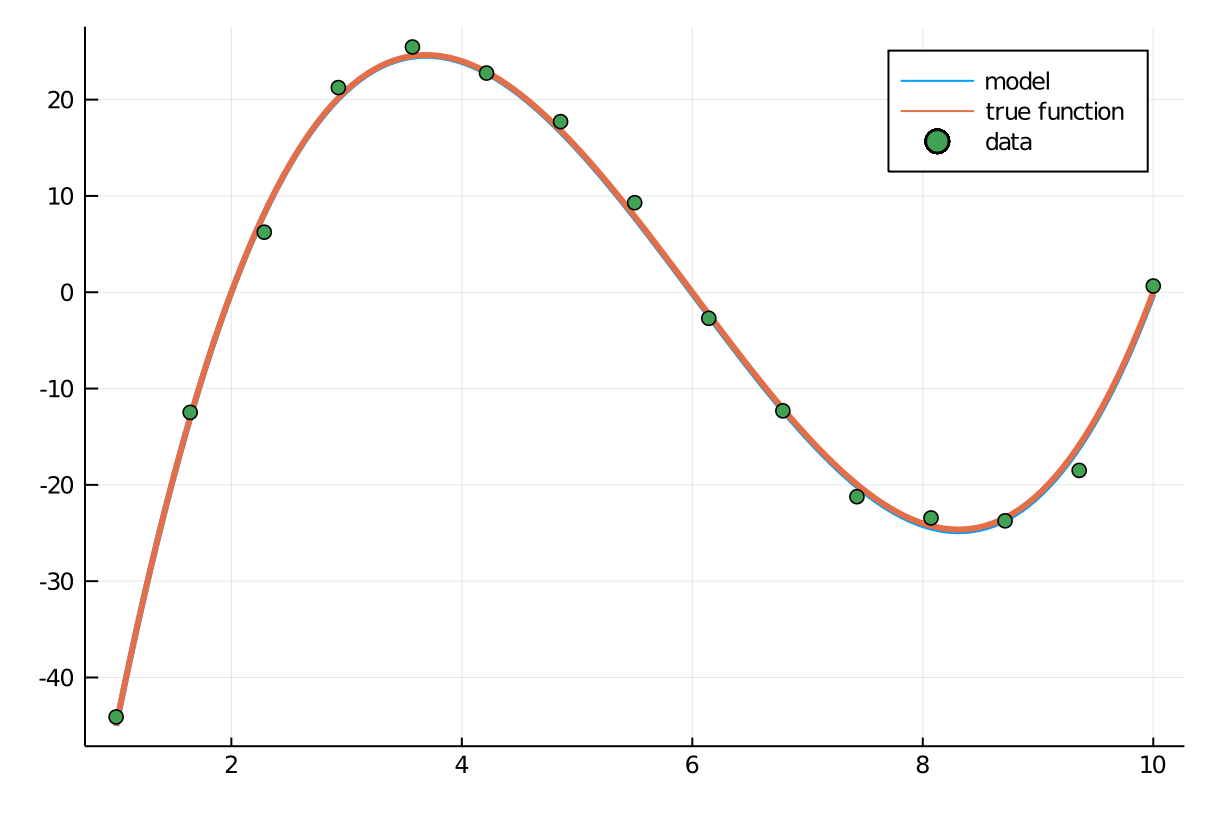
\includegraphics[scale=0.6]{images/courbe1}
\caption{Illustration graphique}
\end{figure}

Ci-dessus, la courbe orange représente le modèle à partit duquel on a généré les données. La courbe bleue, qui colle quasiment parfaitement à l'orange, montre les prédictions du modèle avec $x^{*}$ comme paramètre. Les points verts sont les données perturbées. 

Dans ce cas-ci, on voit que l'on a trouvé les paramètres optimaux.
\newpage
\subsection{Second exemple}

\underline{Vraie fonction} $t\mapsto 1 - \dfrac{t^2}{2} + \dfrac{t^4}{24}$
\newline

\underline{Modèle à ajuster}:

$
\begin{array}{l l l }
g:(t, x_1, x_2) \mapsto 1 + x_1t^2 + {x_2}^3\dfrac{t^4}{3}\\
\text{s.c.}\\
x_1 + 2x_2 = \dfrac{1}{2}
\end{array}
$

On cherche $[-0.5,0.5]$ comme minimum.


Point de départ:
$x_{0} = [1, 0]$

En 9 itérations, on trouve 
 $x^{*} = \begin{pmatrix}
0.71843\\
-0.10921
\end{pmatrix}$

\begin{figure}[!h]
\centering
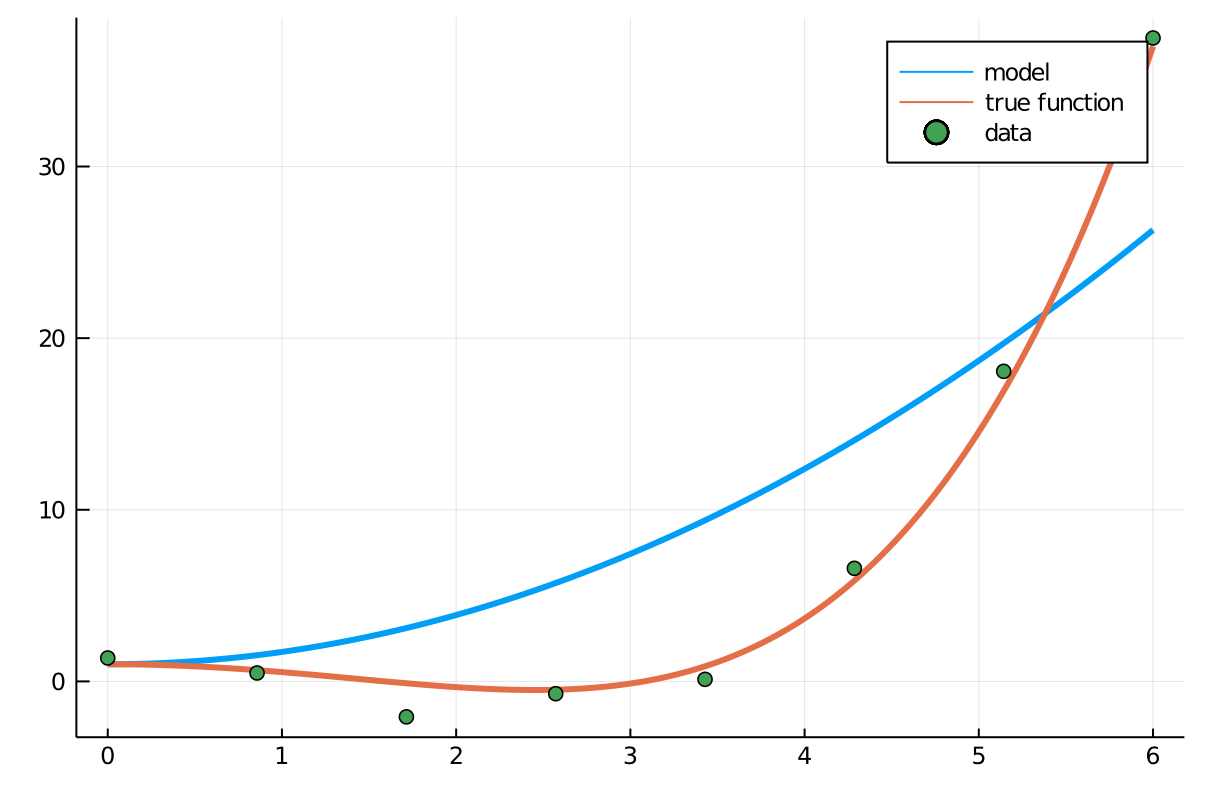
\includegraphics[scale=0.6]{images/courbe2}
\caption{Illustration graphique}
\end{figure}

Ici, la courbe bleue ne correspond pas bien à la courbe orange. Cela illustre le fait que le point trouvé est un minimum local, qui satisfait bien les critères de convergence mais ne correspond pas bien à nos données. 

En changeant le point de départ par $x_{0} = [-0.2,0.1]$, on trouve en 10 itérations:

$$
 x^{*} = \begin{pmatrix}
-0.499987\\
0.50882
\end{pmatrix}$$

Ce résultat, comme le montre l'illustration graphique ci-dessous, est bien plus proche du résultat que l'on souhaite obtenir. Il montre également, bien que le modèle soit simple, la sensibilité au point de départ.
\begin{figure}[!h]
\centering
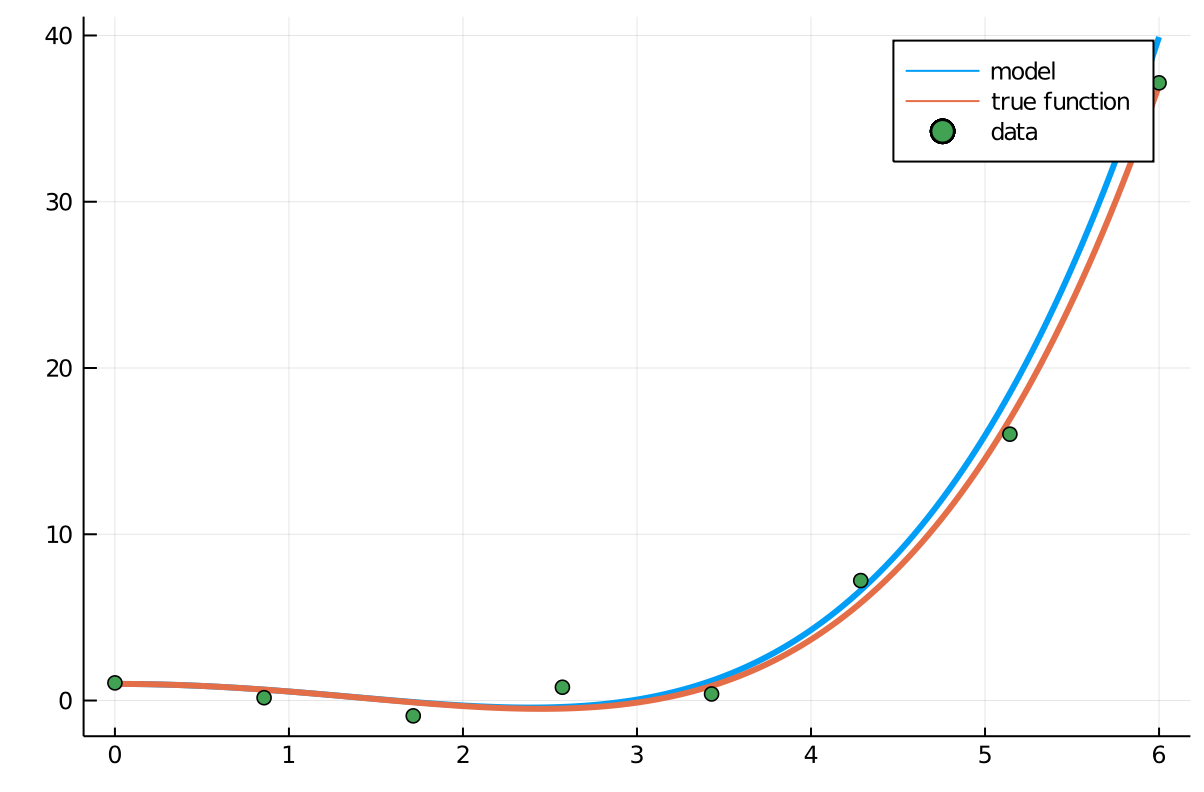
\includegraphics[scale=0.6]{images/courbe3}
\caption{Illustration graphique}
\end{figure}


\bibliographystyle{plain}
\bibliography{biblio_rapport}

\fabian{Fournir les sources BibTeX.}

\end{document}
